\documentclass[conference]{IEEEtran}
\IEEEoverridecommandlockouts
% The preceding line is only needed to identify funding in the first footnote. If that is unneeded, please comment it out.
\usepackage{cite,url}
\usepackage{amsmath,amssymb,amsfonts}
\usepackage{algorithmic}
\usepackage{graphicx}
\usepackage{textcomp}
\usepackage{soul,xcolor}
\usepackage{easyReview}

\usepackage[format=default,justification=centerlast]{caption} % Figure caption text customization

\usepackage[list=true,labelformat=simple]{subcaption}
\renewcommand\thesubfigure{(\alph{subfigure})}
\graphicspath{%
  {figs/matlab/}
}
\def\BibTeX{{\rm B\kern-.05em{\sc i\kern-.025em b}\kern-.08em
    T\kern-.1667em\lower.7ex\hbox{E}\kern-.125emX}}
\begin{document}

\title{Data-Driven Hardware-in-the-Loop Plant Modeling for Self-Driving Vehicles\\
\thanks{This work was partially supported by AutonomouStuff (https://autonomoustuff.com/)}
}


\author{\IEEEauthorblockN{Hannah Grady, Nicholas Nauman, and Md Suruz Miah}
\IEEEauthorblockA{\textit{Department of Electrical and Computer Engineering} \\
\textit{Bradley University}\\
Peoria, Illinois, 61615, USA \\
E-mail: \{hgrady,nnauman\}@mail.bradley.edu, smiah@bradley.edu }
}

\maketitle

\begin{abstract}
\highlight{This report presents the results of modeling vehicle systems and testing them
  using open-loop. First, data was collected for each system using a Lexus
  RX450H vehicle. After data collection, models were developed in order to
  accurately simulate the physical vehicle system. MATLAB's System
  Identification Toolbox was initially used to create these models. However,
the transfer function models it provided w
these systems and their non-linear behaviors. After this was established,
modeling was done using MATLAB's Neural Network Time Series application. Once a
Neural Network model was created, it was then exported to Simulink and modified
to be able to run without the use of the Deep Learning toolbox. These models
gave much more accurate results when compared to the transfer function models
developed using the System Identification Toolbox}

\hl{SM:I'll modify}
\end{abstract}

\begin{IEEEkeywords}
component, formatting, style, styling, insert
\end{IEEEkeywords}

\section{Introduction}
\label{sec:introduction}

%\todo[inline]{NN/HG: Add 2/3 sentences on what motivated the company to model
%  subsystems of autonomous vehicles, Hint: Erik mentioned already that employees
%can perform testing without the physical vehicle. You just need to extend his statement to write the motivational paragraph behind this project}

Due to escalating demand of self-driving vehicles, automotive industry is gradually shifting its attention in  manufacturing a variety of autonomous vehicles. The advancement of new technologies led the automotive industry to develop such vehicles for commercial and personal use as they mainly aim to reduce crashes, energy consumption, pollution, and congestion. However, the development of process of autonomous vehicles still faces signifant challenges to overcome. As it is apparent, each self-driving vehicle is composed of varaious subsystems that researchers of autonomous vehicle community analyze, design, develop, and test.  Intuitively, self-driving vehcles require thorough testing at the factory level before their demonstrations for  the commerical purpose. Such a testing procedure for each physical vehicle is inefficient and costly as it involves testing of different subsystems, such as steering, brake, shift, to name a few, of a vehicle. In this work, we model different modules/subsystems of a self-driving vehicle using machine learning techniques, where a physical self-driving vehicle is not required for testing. Note that modeling vehicle subsystems is a pre-requisite for the development of reliable controllers for autonomous vehicles to be managed in the era of modern transportation systems in general. In particular, modeling different subsystems is conducted for a self-driving vehicle from the vehicle fleet shown in Fig.~\ref{fig:fleet}. %
%
\begin{figure}[htbp]
  \centering
  \includegraphics[scale=0.15]{figs/img/autonomousVehiclesAStuff}
  \caption{Autonomous vehicle fleet (courtesy of AutonomouStuff Inc., https://autonomoustuff.com)}
  \label{fig:fleet}
\end{figure}
%
Such modeling process would allow companies to continue crucial deliveries or transports of their products even if there is a shortage of drivers. %


% \begin{figure}[htbp]
%   \centering
%   \begin{subfigure}[b]{0.48\linewidth}
%     \centering
%        \caption{}
%     \label{fig:fleet}
%   \end{subfigure}
%   \begin{subfigure}[b]{0.48\linewidth}
%     \centering
%
%     \caption{}
%     \label{fig:steerOverview}
%   \end{subfigure}
%   \caption{\subref{fig:fleet} Autonomous vehicle fleet in AutonomouStuff Solutions and \subref{fig:steerOverview} steering model setup (courtesy of AutonomouStuff). }
%   \label{fig:AstuffFleetSteeringSetup}
% \end{figure}


Autonomous vehicles have the ability to make roads safer for drivers
and pedestrians alike. To develop a reliable and safe transportation system for
modern world, a large body of research in the field of autonomous vehicles is
being conducted in recent decades~\cite{Liu2017,Prasad2020}.


Usually, there are six main subsystems of a self-driving vehicle: %
%
\begin{enumerate}
\item  Steering,

\item acceleration,

\item brake,

\item shift,

\item speed, and

\item speed control (cruise).
\end{enumerate}
%
These subsystems are to be modeled to get an accurate representation of how
the vehicle should be controlled. Within the scope of this project and to expedite the modeling process, commercially available modeling tools in Mathworks' MATLAB, System Identification app in the System Identification Toolbox and Neural Network Time Series app in the Deep Learning toolbox, were used to model six subsystems for a Lexus vehicle platform, which is an experimental autonomous vehicle platform that belongs to AutonomouStuff Solutions~\footnote{\url{https://autonomoustuff.com/}}. By creating these software models, the company can run tests using them without needing the physical vehicle. As a result, these models could potentially allow the company to get more testing done.

The first subsystem we will model is the steering model, and then we will move onto
the other subsystems. There are already controllers in place for the Lexus
vehicle platform, but their ability to match the desired input specified by the vehicle operator
%\comment{reliability}{Need to define what do you mean by reliability, be very specific}
is lower than expected due to non-linear
behaviors of the torque voltages required to control each subsystem. The scope
of this project includes developing mathematical and/or data-driven models for each subsystem so that one can easily implement control systems that improve the reliability of the
autonomous vehicle platform. These models will be considered reliable if they can track actual vehicle subsystem behaviors with a minimum best fit percentage between 85 to 95 percent and fall within the error bounds defined for each subsystem. Once these models are developed, they will be tested using Hardware-in-the-Loop (HIL) bench.
Once there is confidence in each model, these models can be used on the   HIL bench to develop controllers that will remove the non-linear behaviors of each vehicle subsystem.
\section{Self-Driving Vehicle Overview}
\label{sec:selfDrivingVehicleOverview}
In this section, we present an overview of the self-driving vehicle pertaining to the hardware-in-the-loop modeling process conducted in the work.

There are two operating modes of the Lexus vehicle platform used in this project: %
%
\begin{itemize}
  \item Manual-drive and
  \item by-wire or autonomous.
\end{itemize}
%
Manual-drive operation occurs when the driver has complete control over the vehicle, including controlling the steering, speed, acceleration, and braking of the vehicle. Autonomous operation occurs where the vehicle is controlled by a computer under driver supervision.
%
Fig.~\ref{fig:steerOverview} depicts how the by-wire mode controls the vehicle. Each
subsystem, like the steering system in this example, sends torque voltages to a
motor that will control the subsystem. %
%
\begin{figure}[htbp]
  \centering
  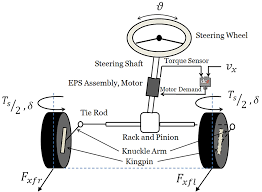
\includegraphics[scale=0.8]{figs/img/autonomousVehiclesSteering}
  \caption{Steering subsystem in autonomous mode (courtesy of Autonomoustuff.com).}
  \label{fig:steerOverview}
\end{figure}
%
In Fig.~\ref{fig:steerOverview}, the motor would
turn the pinion arms which would change the steering angle of the vehicle. The idea of by-wire mode for other vehicle subsystems is controlled in a similar manner with torque voltages being applied to a motor that controls the vehicle subsystem.




\vspace*{12pt}




\section{Conclusion and Future Work}
\label{sec:conclustionAndFutureWork}
Our initial approach was to model the subsystems using the System Identification Toolbox from MATLAB, but it produced unsatisfactory results. Switching to the Neural Network Time Series app allowed us to train models using the data we collected. These models that were developed met the predefined accuracy requirements, and so were tested using an open loop setup. In the future if AutonomouStuff would like to model other vehicle subsystems, we would recommend modeling them using Neural Networks. Creating the Neural Networks and exporting the models to Simulink was easy to do and produced accurate results.

For this project, further testing should be completed for these subsystem models. Since time and availability constraints prevented us from testing the models using Hardware-in-the-Loop, this would be a good place to start. Further testing is important to make sure the developed models are accurate and compatible with testing using hardware. Depending on what AutonomouStuff decides, future engineers working on this project could start developing controllers based off of these models. Currently, AutonomouStuff develops their own controllers for their vehicle subsystems, but they could allow students to design some as part of this senior project.

\bibliographystyle{IEEEtran}
\bibliography{bib/references.bib}

\end{document}
